\documentclass[aspectratio=169, 12pt, final]{beamer}
\usepackage{caption}
\captionsetup[table]{labelformat=empty}
\usepackage{graphicx}

\setbeamertemplate{navigation symbols}{}
\setbeamertemplate{caption}[numbered]

\usepackage[utf8]{inputenc}
\usepackage{enumerate}
\usepackage{tikz}
\usepackage{adjustbox}
\usepackage{marvosym}

\usetheme{default}


\usefonttheme[onlymath]{serif}%makes the math look right;

\usepackage{graphicx}
\usepackage{overpic}
\usepackage{transparent}
\usepackage{multirow}
\usepackage{colortbl}
%\usepackage[eurosym]{eurofont}
\usepackage{caption}
%\usepackage[table]{xcolor}
\usepackage[font=scriptsize,labelfont=bf]{caption}
\usepackage{sidecap}
\usepackage{booktabs}


%\DeclareCaptionFont{blue}{\color{blue}}
%\captionsetup{labelfont={blue,bf}}
\usepackage{booktabs}
\usepackage{centernot}


\title{The Rise of American Ingenuity: Innovation and Inventors in the Golden Age \\
Akcigit, Grigsby, Nicholas (2017)}
\author{Jeanne Sorin}
\date{January 2021}




\begin{document}

\frame{\titlepage}


\begin{frame}
\frametitle{Motivations}
Background
\begin{itemize}
	\item Innovation and technological progress at the core of endogenous growth literature
\end{itemize}
Filling the Gap
\begin{itemize}
	\item Long Run evidence missing because of data limitation
\end{itemize}
\end{frame}


\begin{frame}
\frametitle{Contributions}
\begin{itemize}
	\item A unique dataset : Comprehensive US patents (6 million patents) between 1880 and 1940 at the level of the individual inventor, matched to US Census Data (46 percent match)
	\begin{itemize}
		\item Patents: commonly used measure of innovation
		\item Low access cost to patenting: key to the approach
	\end{itemize}
	\item A Framework for Analyzing Key macro and micro-level determinants
	\begin{enumerate}
	\item At the state level (macro): examine population density, financial development, geographical connectedness, social structure
	\begin{itemize}
		\item Instrument Variables to reveal the causal effect of invention on growth: OSRD contracts for wartime technological development
	\end{itemize}
	\item At the inventor level (micro): examine life cycle, education and migration decisions
\end{enumerate}
\end{itemize}
\end{frame}


\iffalse

\begin{frame}
\frametitle{Main Findings}
\begin{itemize}
	\item \textbf{Regional Facts}: positive impact of invention on growth (could this be endogenous?), more inventive states are densely populated, financially-developed, geographcially connected.
	\item \textbf{Personal Facts}: inventors were more educated, fewer children, more likely to have migrated
	\item \textbf{Family Background}: inventors were more likely to have a high father's income, education
	\item \textbf{The Returns to Innovation}: higher labor income
	\item \textbf{Inequality and Social Mobility}: lower inequality and higher mobility foster invention
\end{itemize}
\end{frame}
\fi

\begin{frame}
\frametitle{Main Findings}
\begin{figure}
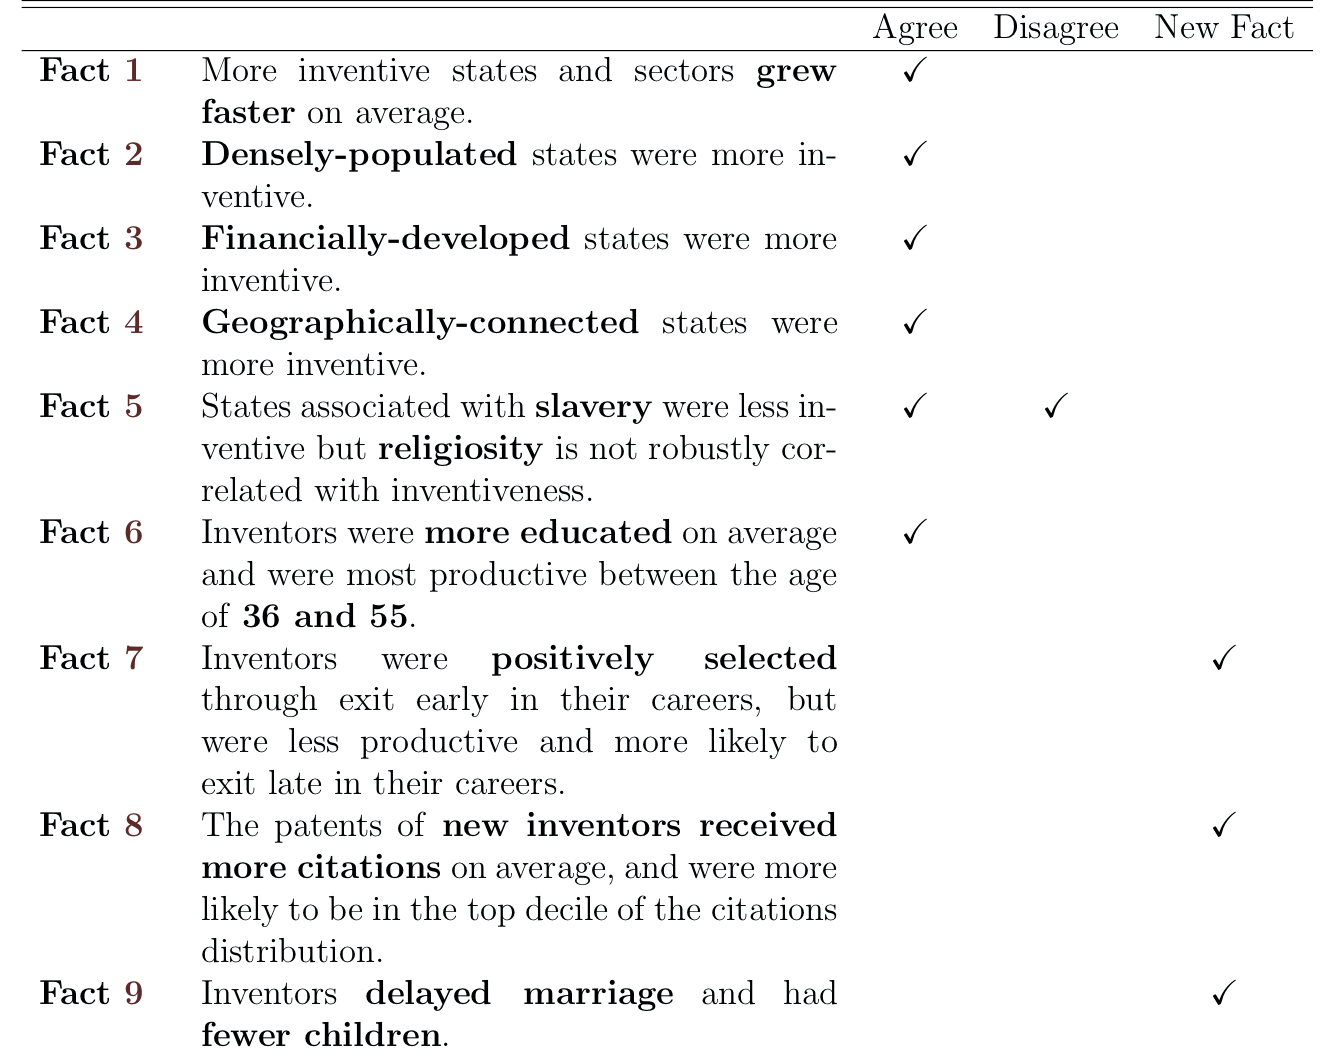
\includegraphics[width=9cm]{W1_Table19_part1.jpeg}
\end{figure}
\end{frame}
\begin{frame}
\frametitle{Main Findings}
\begin{figure}
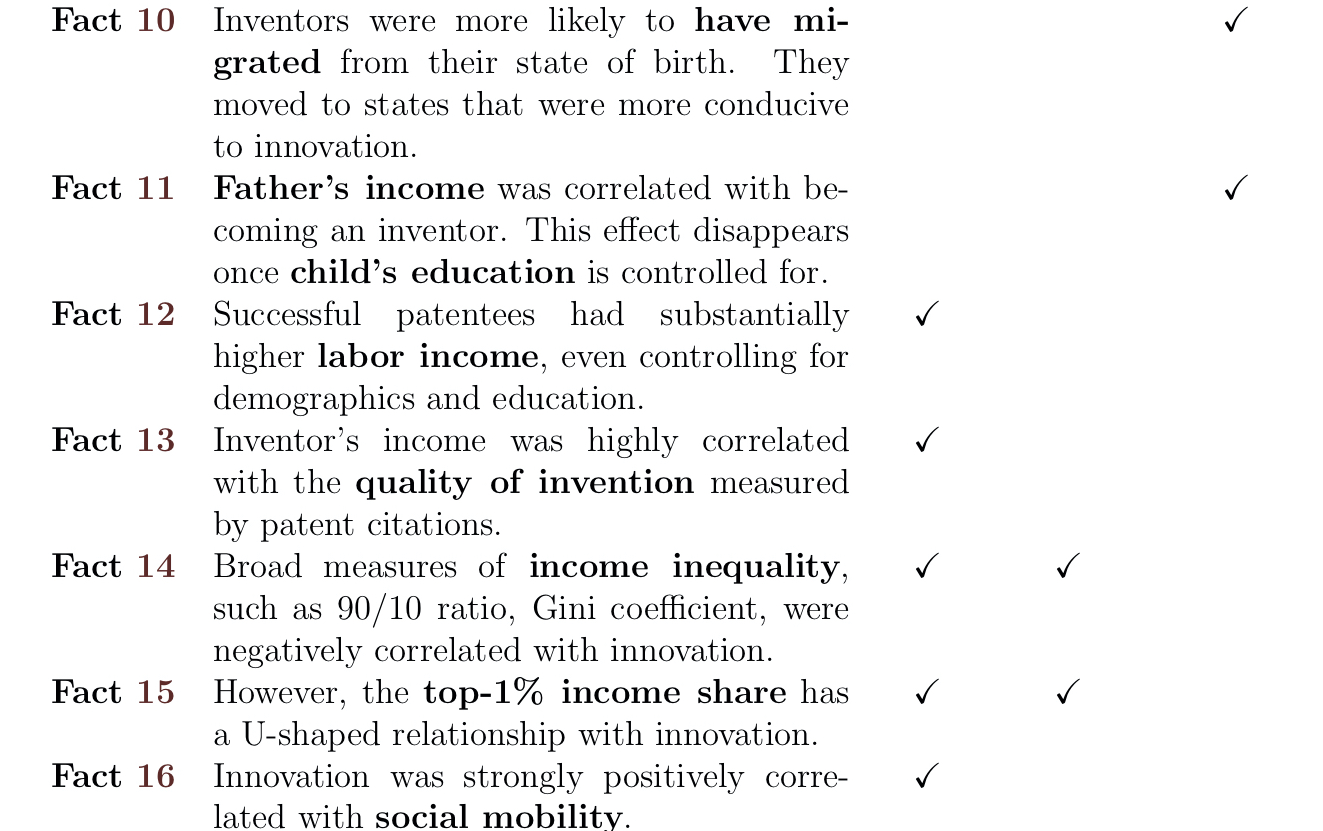
\includegraphics[width=9cm]{W1_Table19_part2.jpeg}
\end{figure}
\end{frame}

\begin{frame}
\frametitle{For myself (not keep)}
Findings interpretations
\footnotesize
\begin{itemize}
	\item 1 Contribution : provided empirical evidence. Estimate suggest that if MA and WY have the same GDP per capita in 1900 and pop density, in 2000, MA would be 30\% richer than WY just because differences in innovativeness. OSRD contracts for wartime techno development as an instrument for innovation
	\item 2 A one standard deviation increase in the percent of a pop living in an urban area is associated with an increase in innovation that is 41.5\% of its mean.
	\item 3 Financial development as bank deposits per capita in 1920
	\item 4 Geographic connectivity may increase innovation both by allowing inventors to sell their inventions to a larger market, and by encouraging the fre exchange of ideas across geographies. Positive relationship holds for non-western states, that had much lower transporation costs in general
	\item 5 Wright (1986) for the slavery argument, Weber (ascetic protestanism) for the religion argument. See Benabou's literature (negative relationship between religiosity and innovation in the US)
	\item 6 Straightforward
	\item 7 Same
\end{itemize}
\end{frame}
\begin{frame}
\frametitle{For myself (not keep)}
Findings interpretations
\footnotesize
\begin{itemize}
	\item 8 Same
	\item 9 Same
	\item 10 Same
	\item 11 Capturing only inventors early in their career because must be same household. \\ Potential mechanisms: wealth of parents, credit constraint, better-connected social circles, useful skills from parents. When including the child's own eduaion, the effect of parental income disappears, suggesting that parental income only positively affects the proba of becoming an inventor through its effect on children's access to education
	\item 12 Straightforward
	\item 13 One the one hand, if innovation dislaces incumbent firms and creates new wealth for competing entrants, more innovative societies are more likely to have lower income inequality (Jones and Kim). However, if innovation primarily strengthens incumbent firms, allowing them to increase markups and constrain output, income inequality in a society may rise with its level of innovation.
	\item 14 Straightforward
	\item 15 Negative relationship patents and top 1\% income in the least productive states, positive in the most.
	\item 16 The Schumpetarian paradigm suggests that innovation allows a new entrant to capture markets for old incumbents. This process of creative destruction creates churn in the economy, allowing individuals and firms with limited market shares to grow.
\end{itemize}
\end{frame}


\begin{frame}
\frametitle{Remaining Questions / Comments}
\begin{itemize}
	\item Macro level: The OSRD IV tries to make the case from correlation to causality of invention on growth. Why is this result not more emphasized in the framing of the paper?
	\item Data: Are the sample of matched / unmatched inventors (to Census data) \textit{``balanced''}? Across states?
	\item Policy: How to interpret the findings (especially macro ones) in light of policy?
	\item Is there any \textit{``path dependence''} and peer effects: do inventors live in states with more inventors, \textit{ceteris paribus}?
	\item Methodology: Why favor state level over county level for the main analysis?
	\item What about the role of major (scientific) schools?
\end{itemize}
\end{frame}



\end{document}